\chapter{Stand der Technik}
\section{Straßenschilderkennung}
\label{chap:stand-der-technik-strassenschilderkennung}
Eine Straßenschilderkennung zählt mittlerweile zu der Standardausstattung vieler Neuwagen. Im Jahr 2024 tritt zudem eine EU-Verordnung in Kraft, durch die sämtliche neu produzierten Fahrzeuge mit einer solchen Funktion ausgestattet werden müssen \cite{eu-regulation}. Daran zeigt sich, dass das Thema bereits weitreichend etabliert ist.

Straßenschilder werden zu folgendem Zweck eingesetzt: Es sollen Informationen über die Verkehrssituation und über geltende Vorschriften des Gebiets, in dem sich das Fahrzeug zu einem gegebenen Zeitpunkt befindet, präsentiert werden. Durch Straßenschilder werden unter anderem Geschwindigkeitsvorgaben, Gefahrenhinweise und allgemeine Verkehrsregeln kommuniziert. Dabei sind die Schilder so konzipiert, dass sie sich visuell möglichst von ihrem Hintergrund abheben und leicht voneinander zu unterscheiden sind. Automatische Straßenschilderkennungen können Fahrer*innen in Situationen unterstützen, in denen sie Schilder übersehen oder gezielt missachten. Anstelle dass ein reales Schild beispielsweise nur für einige Sekunden sichtbar ist, bevor es außerhalb der Sichtweite des Fahrzeugführenden ist, ist eine durchgehende Anzeige auf den Displays eines Fahrzeugs möglich. Auch akustische Warnungen oder ein aktives Eingreifen von Sicherheitssystemen sind denkbar, beziehungsweise bereits in Serienfahrzeugen vorhanden.

Eine Straßenschilderkennung erfolgt visuell und wird somit mittels Kameras umgesetzt. Dabei lassen sich viele Schilder durch eine bestimmte Form (Kreis, Dreieck, Achteck, etc.) und ein Piktogramm (Schneeflocke, Person, etc.) oder eine Zahl identifizieren. Somit können die verschiedenen Arten von Straßenschilder in Klassen unterteilt werden, die durch den Erkennungsalgorithmus detektiert werden. Für die praktische Umsetzung solcher Algorithmen werden häufig \acp{KNN} verwendet. Diese werden in Kapitel \ref{chap:KNNs} thematisch aufgeführt. Besonders relevant für das Thema dieser Studienarbeit ist, wie zuverlässig die momentan ausgelieferten Straßenschilderkennungen sind und welche Situationen die Algorithmen am ehesten zu falschen Aussagen verleiten. Auf dieser Grundlagen kann sich orientiert werden, welche Arten von Bildern vermehrt generiert werden sollen, um die Straßenschilderkennung verbessern zu können.

Im Jahr 2019 hat eine Automobilzeitschrift die Straßenschilderkennung von unterschiedlichen Fahrzeugherstellern getestet \cite{strassenschilderkennungTest}. Zudem existieren verschiedene Publikationen, die sich mit der Thematik befassen \cite{traffic-sign-detection-review-2014}. Die Ergebnisse des Zeitschriftenartikels weisen darauf hin, dass die Straßenschilderkennung einiger Fahrzeuger bereits weitreichend funktioniert. Geschwindigkeitsvorgaben werden überwiegend erkannt und dem Fahrer auf einem Display angezeigt. Auch existieren bereits akustische Warnungen bei einer Überschreitung der Höchstgeschwindigkeit. Dennoch existieren einige Situationen, die bei mehreren Fahrzeugen zu Problemen bei der Straßenschilderkennung geführt haben. Einen exemplarischen Überblick soll die folgende Grafik bieten: \cite{strassenschilderkennungTest} 

\begin{figure}[H]
   \centering
   \captionsetup[subfigure]{labelformat=empty}
   \begin{subfigure}[b]{0.125\textwidth}
       \centering
       \includegraphics[height=\textwidth]{../images/Schilder Beispiele/Aufhebungsschild.png}
       \caption{Aufhebung}
       \label{fig:aufhebungsschild}
   \end{subfigure}
   \hspace{3em}%
   \begin{subfigure}[b]{0.125\textwidth}
       \centering
       \includegraphics[height=\textwidth]{../images/Schilder Beispiele/Abgeklebt.jpg}
       \caption{Ungültigkeit}
       \label{fig:abgeklebt}
   \end{subfigure}
   \hspace{3em}%
   \begin{subfigure}[b]{0.125\textwidth}
       \centering
       \includegraphics[height=\textwidth]{../images/Schilder Beispiele/Dunkelheit.png}
       \caption{Dunkelheit}
       \label{fig:dunkelheit}
   \end{subfigure}
   \hspace{3em}%
   \begin{subfigure}[b]{0.125\textwidth}
    \centering
    \includegraphics[height=\textwidth]{../images/Schilder Beispiele/Wechselverkehrszeichen.jpg}
    \caption{LED Schilder}
    \label{fig:ledschild}
   \end{subfigure}
      \caption{Erschwerende Einflüsse auf die Straßenschilderkennung \cite{GTSRB}}
      \label{fig:einfluesse-strscherkennung}
\end{figure}

Fahrzeuge verschiedener Hersteller haben in den Tests Aufhebungsschilder nicht korrekt interpretiert. Damit sind Schilder gemeint, die entweder Geschwindigkeitsbegrenzungen oder Überholverbote außer Kraft setzen. Des Weiteren sorgten mittels Klebestreifen als ungültig erklärte Schilder, in einigen Fällen Dunkelheit, beispielsweise in Tunneln, und sogenannte LED \emph{Wechselverkehrszeichen} für falsche Aussagen. Auch wird teilweise nicht erkannt, wenn Schilder für eine kreuzende Straße gelten, statt für die Straße, auf der sich das Fahrzeug zu dem gebenen Zeitpunkt befinden. Weitere Aspekte, die in dem Artikel nicht explizit genannt sind, aber laut einer Publikation von 2014 in der Vergangenheit zu Schwierigkeiten geführt haben, sind mitunter die folgenden: \cite{traffic-sign-detection-review-2014}

\begin{figure}[H]
   \centering
   \captionsetup[subfigure]{labelformat=empty}
   \begin{subfigure}[b]{0.125\textwidth}
       \centering
       \includegraphics[height=\textwidth]{../images/Schilder Beispiele/Schnee.jpg}
       \caption{Witterung}
       \label{fig:witterung}
   \end{subfigure}
   \hspace{3em}%
   \begin{subfigure}[b]{0.125\textwidth}
       \centering
       \includegraphics[height=\textwidth]{../images/Schilder Beispiele/MotionBlur.png}
       \caption{Unschärfe}
       \label{fig:motion-blur}
   \end{subfigure}
   \hspace{3em}%
   \begin{subfigure}[b]{0.125\textwidth}
       \centering
       \includegraphics[height=\textwidth]{../images/Schilder Beispiele/Überbelichtung}
       \caption{Belichtung}
       \label{fig:ueberbelichtung}
   \end{subfigure}
   \hspace{3em}%
   \begin{subfigure}[b]{0.125\textwidth}
    \centering
    \includegraphics[height=\textwidth]{../images/Schilder Beispiele/Vandalismus.png}
    \caption{Vandalismus}
    \label{fig:vandalism}
   \end{subfigure}
      \caption{Weitere mögliche Einflüsse auf die Straßenschilderkennung}
      \label{fig:einfluesse-strscherkennung2}
\end{figure}

Eine weitere Publikation aus dem Jahre 2019 zeigt, dass die Qualität der Straßenschilderkennung von der Stärke der äußeren Einflüsse abhängt. Vergleichsweise geringfügig verdeckte Schilder hat das Testfahrzeug hier beispielsweise in der Regel korrekt klassifizieren können. Sobald eine größere Fläche des Schild verdeckt ist oder das Schild vermehrt beschmutzt ist, ist keine korrekte Klassifizierung erfolgt. Auch hier schreiben die Autoren, dass das Wetter und somit Sichtverhältnisse einen negativen Einfluss auf die Qualität der Erkennung zeigen. \cite{traffic-sign-anomalies}

Die Erkenntnisse der Tests aus den genannten Artikeln geben Hinweise auf das folgende: In einigen genannten Situationen können sich die Fahrzeugführenden nicht vollständig auf die Straßenschilderkennung ihrer Fahrzeuge verlassen. Ein Ziel der Hersteller ist das Anbieten von Fahrzeugen, die vollständig autonom, das heißt ohne menschliches Eingreifen, fahren können. Damit das möglich ist, muss die Software der Fahrzeuge auch solche Grenzfälle korrekt interpretieren. Das erfordert eine gewisse Menge an Daten, durch die diese Algorithmen trainiert werden.

Ziel dieser Arbeit ist ausgehend davon, gezielt Trainingsbilder erzeugen zu können, die einige dieser Aspekte simulieren. Es soll als alternative Möglichkeit dazu vorgeschlagen werden, sämtliche Trainingsdaten für Grenzfälle eigenständig in realen Fahrsituationen aufzunehmen.

%Diese EU-Verordnung verfolgt im wesentlichen das Ziel, verschiedene sicherheitsrelevante Systeme verpflichtend %einzuführen. Dazu zählen zudem Notbremsassistenten, Müdigkeitswarner und Notbremslichter. Die %Straßenschilderkennung trägt dazu im wesentlichen durch die Möglichkeit einer Warnung bei überhöhter %Geschwindgkeit oder einer automatischen Geschwindigkeitsanpassung bei.

\section{Künstliche Neuronale Netze}
\acused{KNN}
\label{chap:KNNs}
Durch künstliche neuronale Netze (\acsp{KNN}) können Maschinen lernen, bestimmte Probleme zu lösen, ohne dass ein Mensch vorher explizite Regeln dafür definieren muss. Dies steht im Kontrast zur Methode, der Maschine  vorher einen festen, vollständigen Regelsatz bereitzustellen. Letztgenannter Ansatz zeigt in einigen Gebieten nur begrenzten Erfolg, da es für Menschen herausfordernd sein kann, Regelsätze für Vorgänge zu definieren, die unbewusst im Gehirn stattfinden oder viel Kontext erfordern. Zu nennen sind hierbei die visuelle Objekterkennung oder menschliche Sprache. Außerdem können neue, nicht in den Regeln beachtete Situationen dazu führen, dass die Maschine das Problem nicht mehr lösen kann. \cite{DeepLearningBook}

Die Grundidee hinter dem sogenannten \emph{maschinellen Lernen} ist deshalb, dass sich die Maschine selber einen Wissensschatz aufbaut, der ihr beim Lösen des Problems hilft. Dies geschieht, indem die Entwickler ihr reale Trainingsbeispiele zeigen. Möchte man einen Algorithmus trainieren, der Schach spielen soll, kann man ihm beispielsweise eine Vielzahl an realen Schachpartien zeigen. Anhand dessen lernt der Algorithmus verschiedene Strategien und baut ein Spielverständnis auf, das womöglich über die menschlichen Fähigkeiten hinausgeht. \acp{KNN} bauen auf diesem Prinzip auf. Sie implementieren lernbare Funktionen, die eine Abbildung zwischen einer Eingabe und der zugehörigen Ausgabe herstellen. \cite{DeepLearningBook}

In den letzten Jahrzehnten erlebte das maschinelle Lernen und damit auch das Gebiet der \acp{KNN} einen Aufschwung. Es existiert bereits seit Mitte des vergangenen Jarhunderts, wird allerdings erst durch die zunehmende Rechenleistung und die Verfügbarkeit von großen Datenmengen flächendeckend eingesetzt. Einsatzgebiete für \acp{KNN} sind unter anderem die Objekterkennung, das Verstehen von natürlicher Sprache und die Generierung von Text und Bildern. \cite{knnsKompakt}

Die Inspiration für \acp{KNN} bildet die Informationsverarbeitung des Gehirns in Lebewesen. Die kleinste hier betrachtete Einheit ist das Neuron. Neuronen in \acp{KNN} sind konzeptionell inspiriert von realen, biologischen Neuronen, besitzen aber eine abstrahierte Funktionsweise. In \acp{KNN} berechnen sie ein Skalarprodukt ihrer gewichteten Eingangswerte, addieren einen sogennaten \emph{Schwellenwert} (\emph{engl.: Bias}) hinzu und wenden auf das Ergebnis eine nichtlineare Funktion an. Letzere wird auch als Aktivierungsfunktion bezeichnet. 
Diese Aktivierungsfunktion kann analog dazu gesehen werden, dass biologische Neuronen einen Grenzwert (\emph{engl.: threshold}) besitzen, der überschritten werden muss, damit das Neuron \emph{feuert}, also einen Impuls an weitere Neuronen weitergibt. Aktivierungsfunktionen sind notwendig, damit neuronale Netze Probleme lösen können, die über die Fähigkeiten einer linearen Regression hinausgehen. Dadurch können Neuronen eine nichtlineare Abhängigkeit zwischen dem Eingang $x$ und dem Ausgang $y$ umsetzen. \cite{visualApproach}

In Abbildung \ref[fig:neuron] ist ein einzelnes künstliches Neuron eines \acp{KNN} darstellt. Das \emph{Plus-Zeichen} steht für die Berechnung des Skalarprodukts der Eingänge und der darauf addierte Schwellenwert. Die Aktivierungsfunktion wird durch das \emph{Sigmoid}-Zeichen simbolisiert. Der Ausgang (\emph{rechts}) ist das Ergebnis der Berechnung des Neurons. \cite{visualApproach}

\begin{figure}[H]
   \centering
   \includegraphics[width=0.4\textwidth]{images/KNNs/Neuron.png}
   \caption{Einzelnes Neuron eines \acp{KNN} \cite{visualApproach}}
   \label{fig:neuron}
\end{figure}

Um komplexe Probleme lösen zu können, besitzen \ac{KNN} mehrere Neuronen, die miteinander verbunden und in Schichten angeordnet sind. Jede Schicht erhält die Ausgangswerte der vorherigen Schicht als Eingang und gibt die daraus berechneten, neuen Werte an die nächste Schicht weiter. Abbildung \ref{fig:KNN} zeigt ein vollständiges \ac{KNN}. Die Neuronen sind durch Kreise dargestellt und ihre Verbindungen durch Pfeile. \cite{knnsKompakt} 

\begin{figure}[H]
   \centering
   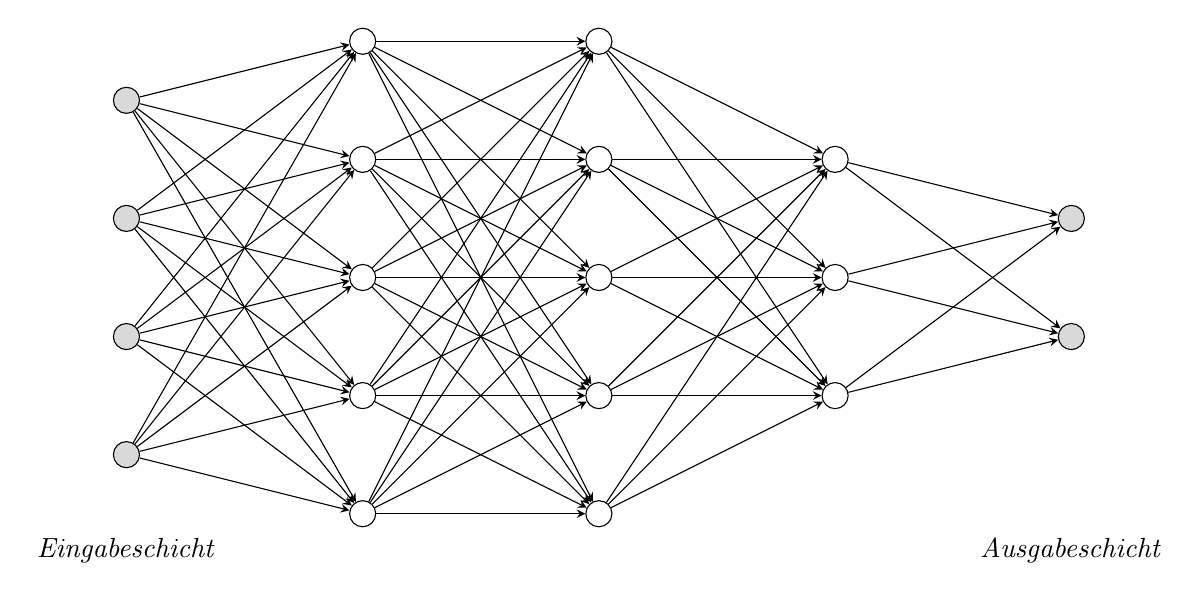
\begin{tikzpicture}[x=1.5cm, y=1.5cm, >=stealth]
      % Input layer
      \foreach \i in {1,...,4}
      \node[circle, draw=black, fill=gray!30] (in-\i) at (0,\i-2) {};
      
      % Hidden layer 1
      \foreach \i in {1,...,5}
      \node[circle, draw=black, fill=white] (h1-\i) at (2,\i-2.5) {};
      
      % Hidden layer 2
      \foreach \i in {1,...,5}
      \node[circle, draw=black, fill=white] (h2-\i) at (4,\i-2.5) {};

      % Hidden layer 3
      \foreach \i in {1,...,3}
      \node[circle, draw=black, fill=white] (h3-\i) at (6, \i-1.5) {};
      
      % Output layer
      \foreach \i in {1,...,2}
      \node[circle, draw=black, fill=gray!30] (out-\i) at (8,\i-1) {};
      
      % Connections
      \foreach \i in {1,...,4}
      \foreach \j in {1,...,5}
      \draw[->] (in-\i) -- (h1-\j);
      
      \foreach \i in {1,...,5}
      \foreach \j in {1,...,5}
      \draw[->] (h1-\i) -- (h2-\j);

      \foreach \i in {1,...,5}
      \foreach \j in {1,...,3}
      \draw[->] (h2-\i) -- (h3-\j);
      
      \foreach \i in {1,...,3}
      \foreach \j in {1,...,2}
      \draw[->] (h3-\i) -- (out-\j);
      
      % Labels
      \node[above] at (0,-2) {\emph{Eingabeschicht}};
      \node[above] at (8,-2) {\emph{Ausgabeschicht}};
      
   \end{tikzpicture}
		\caption{Vollständiges \ac{KNN} \emph{(angelehnt an \cite{visualApproach})}}
      \label{fig:KNN}
\end{figure}

Eine Verbindung stellt dar, dass ein Neuron seinen berechneten Wert an das nachfolgende Neuron weitergibt. Dies geschieht hierbei ausschließlich von \emph{links nach rechts}, womit das \ac{KNN} als \emph{Feedforward-Netzwerk} bezeichnet wird. Die Eingabeschicht erhält die Eingabewerte des Netzwerks, die Ausgabeschicht liefert die Vorhersage des Modells. Zwischen diesen beiden Schichten befinden sich beliebig viele verarbeitende Schichten, die als \emph{Hidden Layer} bezeichnet werden. Die Neuronen der Hidden Layer sind in Abbildung \ref{fig:KNN} in weiß dargestellt. \cite{knnsKompakt}

Die Vorhersage, gekennzeichnet durch die Werte der Ausgabeschicht, hängt von den jeweiligen Parametern der Neuronen des Netzwerks ab. Dies sind die Gewichte (\emph{engl.: weights}) der Verbindungen zwischen den Neuronen sowie der Schwellenwert der Neuronen. Es existieren auch trainierbare Aktivierungsfunktionen, diese sind jedoch vergleichsweise unüblich. Entwickler sind für den Entwurf der Netzwerkarchitektur zuständig, die Parameter werden jedoch durch das Modell trainiert. Zu Beginn besitzt das Modell zufällige Parameter, wodurch es in der Regel nicht die gewünschte Abbildung zwischen Ein- und Ausgabe implementiert. Ein untrainierter Schachalgorithmus spielt demnach augenscheinlich willkürliche Züge. Ein untrainierter Katzenklassifikator besitzt keinen erkennbaren Wissensschatz darüber, welche Charakteristiken eine Katze optisch auszeichnen. Das Ziel des Trainings ist, dass die Parameter des Modells zunehmend gegen das Optimum konvergieren und so das Modell immer plausibler in seinen Vorhersagen wird. \cite{knnsKompakt} \cite{visualApproach}

%---------------------------------------------------------------------------------------------------------------
\subsection{Training}
Das Training von \acp{KNN} benötigt Daten. Zum einen ein Satz an \emph{Trainingsdaten} und zum anderen ein Satz an \emph{Testdaten}. Die Trainingsdaten dienen dazu, das Modell zu verbessern. Eine \emph{Kostenfunktion} berechnet, wie genau die Vorhersagen des Modells auf den Trainingsdaten sind. Darauf basierend wird das Modell optimiert. Die Testdaten dienen zur Messung der Qualität des Modells. Es kann nämlich vorkommen, dass das \ac{KNN} die Trainingsdaten \emph{auswendig} lernt und deshalb hier gute Ergebnisse erzielt, aber eine unzureichende Performanz auf den Testdaten zeigt. Etwa wenn das \ac{KNN} unerwartete Eigenschaften in den Trainingsdaten lernt. Aus diesem Grund werden trainierte Modelle anhand der Testdaten evaluiert. \cite{knnsKompakt}

Die Kostenfunktion bestimmt die durchschnittliche Fehlerrate des \ac{KNN} auf einem gegebenen Datensatz. Sie berechnet somit, gemittelt über alle $m$ Beispiele aus dem Datensatz, die Abweichung des vorhergesagten Wertes $\hat{y}$ von dem tatsächlichen Wert $y$. Für ein einzelnes Beispiel aus dem Datensatz nutzt die Funktion dafür eine \emph{Verlustfunktion} $\mathcal{L}$. Die Verlustfunktion bewertet somit eine einzelne Aussage des \ac{KNN}, während die Kostenfunktion die durchschnittliche Qualität der Aussagen auf dem gesamten Datensatz misst. Folgende Gleichung zeigt die Kostenfunktion: \cite{DeepLearningBook}

\begin{equation}
   \label{eq:costFunctionGeneral}
   J(\theta) = \frac{1}{m} \sum_{i=1}^{m} \mathcal{L}(\hat{y}^{(i)}, y^{(i)})
\end{equation}
Wobei: \newline
\emph{\null\quad\quad $J$: Wert der Kostenfunktion \newline
\null\quad\quad $\theta$: Trainierbare Parameter des Modells \newline
\null\quad\quad $m$: Anzahl der Trainingsbeispiele \newline
\null\quad\quad $i$: Index des momentan betrachteten Trainingsbeispiels \newline
\null\quad\quad $\mathcal{L}$: Verlustfunktion \newline
\null\quad\quad $\hat{y}$: Vorhersage des Modells \newline
\null\quad\quad $y$: Erwarteter Wert}

Die Kostenfunktion $J$ ist abhängig von einem $\theta$. Das $\theta$ ist ein Vektor, der alle Gewichte und Schwellenwerte und damit alle trainierbaren Parameter des \ac{KNN} beinhaltet. Verändern sich die Parameter des \ac{KNN}, dann liefert es andere Aussagen für das $\hat{y}$. Somit ändert sich der Wert der Kostenfunktion, wenn das \ac{KNN} seine Parameter anpasst.  \cite{DeepLearningBook}

Die Gleichung \ref{eq:costFunctionGeneral} kann auch mit dem Operator $\mathbb{E}$ formuliert werden. Er beschreibt den Erwartungswert: \cite{DeepLearningBook}
\begin{equation}
	\label{eq:costFunctionExpectedValue}
	J(\theta) = \mathbb{E}_{x,y}[\mathcal{L}(f(x; \theta), y)]
\end{equation}
Was in Gleichung \ref{eq:costFunctionGeneral} das arithmetische Mittel der Verlustfunktionen ist, wird hier als Erwartungswert der Verlustfunktion geschrieben. Die Fragestellung lautet: \emph{Wenn ein zufälliges Beispiel $x$ und das zugehörige $y$ aus dem Datensatz gezogen werden, was ist dann der erwartete Verlust des Modells?} Die Vorhersage $\hat{y}$ des \ac{KNN} wird hier als $f(x; \theta)$ geschrieben. Dabei ist $f$ das \ac{KNN}, das für ein gezogenes $x$ eine bestimmte Vorhersage trifft. Diese Vorhersage ist zudem abhängig von $\theta$. Diese alternative Darstellung der Kostenfunktion mit dem Operator $\mathbb{E}$ ist relevant für Kapitel \ref{chap:NoGANs}. \cite{DeepLearningBook}

Kostenfunktionen können verschiedene Arten von Verlustfunktionen verwenden. Für diese Arbeit sind sowohl die $\mathcal{L}_1$ und $\mathcal{L}_2$ Verlustfunktionen als auch der \emph{Binary Crossentropy Loss} von besonderer Relevanz.

\paragraph{$\mathcal{L}_1$ Verlustfunktion} Die $\mathcal{L}_1$ Verlustfunktion berechnet für ein gegebenes Beispiel die absolute Abweichung der Vorhersage von dem erwarteten Wert. Sie wird auch als \emph{mittlere absolute Abweichung} \emph{(engl.: mean absolute error)} bezeichnet.
\begin{equation}
   \mathcal{L}_1 = |\hat{y} - y|
\end{equation}

\paragraph{$\mathcal{L}_2$ Verlustfunktion} Die $\mathcal{L}_2$ Verlustfunktion berechnet hingegen die quadratische Abweichung von dem erwarteten Wert. Hier haben somit größe Abweichungen einen stärkeren Einfluss auf den \emph{Verlust} \emph{(eng.: loss)} als bei der $\mathcal{L}_1$ Funktion. Diese Verlustfunktion wird auch als \emph{mittlere quadratische Abweichung} \emph{(engl.: mean squared error)} bezeichnet.
\begin{equation}
   \mathcal{L}_2 = (\hat{y} - y)^2
\end{equation}

\paragraph{Binary Crossentropy Loss} Die Binary Crossentropy Verlustfunktion ist auch als \emph{logarithmische Verlustfunktion} bekannt. Sie eignet sich für binäre Klassifikationen, wo demnach das \ac{KNN} eine Wahrscheinlichkeit zwischen $0$ und $1$ ausgibt. Ein Beispiel hierfür ist, wenn das \ac{KNN} abschätzen soll, ob auf einem Bild eine Katze zu sehen ist oder nicht. Ein Schwellenwert für eine Wahrscheinlichkeit zwischen $0$ und $1$ gibt dann an, ob das Ergebnis als \emph{Ja} oder \emph{Nein} interpretiert wird. Die Binary Crossentropy Verlustfunktion ist in Gleichung \ref{eq:bce-loss} dargestellt. Die Verlustfunktion nutzt die Eigenschaften aus, dass $\log(1) = 0$ ist und der Logarithmus von Werten zwischen $0$ und $1$ negativ ist. Wenn der erwartete Wert $y$ gleich $1$ ist, dann reduziert sich die Verlustfunktion außerdem zu $\mathcal{L} = -\log(\hat{y})$. Entspricht $\hat{y}$ dem erwarteten Wert von $1$, dann ergibt die Verlustfunktion $-\log(1)=0$. Je weiter $\hat{y}$ gegen $0$ strebt, desto größer wird der Wert für $-\log(\hat{y})$. Ist der erwartete Wert $y$ hingegen gleich $0$, dann reduziert sich die Verlustfunktion zu $\mathcal{L} = -\log(1 - \hat{y})$. Hier tritt der umgekehrte Effekt auf. \cite{bce-loss}
\begin{equation}
	\label{eq:bce-loss}
   \mathcal{L}_{BCE} =  - [y \log(\hat{y}) + (1 - y) \log(1 - \hat{y})]
\end{equation}

Das Training des Modells besteht nicht nur daraus, die Vorhersagen des Modells zu bewerten. Damit das Modell in dem nächsten Trainingsdurchlauf idealerweise einen geringeren Wert für die Kostenfunktion erreicht, müssen die trainierbaren Parameter $\theta$ des Modells angepasst werden. Von ihnen hängt der Wert der Kostenfunktion ab. Die Ausgangssituation ist hierbei die folgende: Mit einem gegebenen $\theta$ befindet sich das \ac{KNN} in einem bestimmten Punkt der Kostenfunktion $J(\theta)$. Gesucht ist eine Parameteränderung $\dif\theta$, mit der sich das \ac{KNN} am weitesten an das globale Minimum der Kostenfunktion annähert. Das globale Minimum ist die beste Lösung, die das Modell für die gegebenen Trainingsdaten finden kann und damit das Optimum. Da $J(\theta)$ eine viel-dimensionale Funktion ist, berechnet die Trainingsfunktion diesen Idealwert für $\theta$ nicht numerisch. Stattdessen nähert sich das \ac{KNN} mit jedem Trainingsschritt dem Optimum an. \cite{knnsKompakt}

Nähern tut sich das \ac{KNN} dem Optimum, indem es den Punkt $\theta$ in Richtung des negativen Gradienten der Kostenfunktion bewegt. Also die Richtung, in die, aus der momentanen Ausgangsposition, die Kostenfunktion den steilsten Abstieg besitzt. Pro Trainingsiteration bewegen sich die Parameter $\theta$ nur um einen kleinen Betrag in Richtung des negativen Gradienten. In einem Trainingsschritt kann das \ac{KNN} auf mehrere annotierte Beispiele trainiert werden. Dann bezieht sich die Verlustfunktion $\mathcal{L}$ nicht mehr nur auf ein einzelnes Trainingsbeispiel, sondern auf einen Teil des gesamten Datensatzes. Die Berechnungsformel ist in dem Fall identisch zu den Kostenfunktionen in Gleichungen \ref{eq:costFunctionGeneral} und \ref{eq:costFunctionExpectedValue}. Das ist relevant für Kapitel \ref{chap:GANs}. \cite{knnsKompakt}

Das Training eines \ac{KNN} wird so lange durchgeführt, bis der Gradient einen so geringen Betrag hat, dass sich die Parameter des \ac{KNN} nicht mehr signifikant verändern. Das \ac{KNN} befindet sich hier bestenfalls im globalen Optimum. Der Betrag der Annäherung pro Trainingsschritt ist durch eine sogennante Lernrate $\alpha$ bestimmt. Die Lernrate ist ein \emph{Hyperparameter}, und damit klassischerweise ein nicht-trainierbarer Parameter, da sie durch die Entwickler fest bestimmt wird und nicht durch das Modell selbst gelernt wird. Ist das \ac{KNN} ein mal mit jedem Trainingsbeispiel trainiert worden, spricht man von einer Trainingsepoche \emph{(kurz: Epoche)}. Üblicherweise werden \acp{KNN} über mehrere Epochen trainiert bis die Parameter des Netzes gegen das Optimum konvergieren \cite{knnsKompakt}

\todo[inline]{Auf Ableitung der Kostenfunktion für Berechnung des Gradienten eingehen?}
\todo[inline]{Hier schon Batches erklären und damit darauf eingehen wie mit einer Verlustfunktion über mehrere Trainingsbeispiele trainiert wird}

%---------------------------------------------------------------------------------------------------------------
\subsection{Convolutional Neural Networks}
\acp{KNN} bewähren sich mitunter besonders im Bereich \emph{Computer Vision}. Ein Bereich, der sich mit der Interpretation von Bild- und Videodaten beschäftigt. Hier spielt die Mustererkennung eine tragende Rolle. Es sollen Merkmale erkannt werden, die jedes Objekt eines bestimmten Typs auszeichnen, die jedoch nicht auf jedem Bild die exakt identischen Pixelwerte besitzen. Die typische Form von Katzenohren ist beispielsweise ein Muster, das bei der Katzenerkennung verwendet werden kann. \cite{knnsKompakt}

Verwendet man hierfür jedoch die bisher beschriebene Netzwerkarchitektur, treten verschiedene Probleme auf. Jedes sogenannte \emph{Merkmal} des Eingangs wird über die Eingangsschicht in das \ac{KNN} gespeist. Bei einem Schachalgorithmus kann die Menge aller Merkmale beispielsweise durch die momentane Position aller Figuren auf dem Schachbrett beschrieben werden. Bei der Bildklassifizierung ist jeder Pixel des Bildes ein Merkmal. Ein Netz, das Bilder der Größe 1024x1024 Pixel mit drei Farbkanälen (rot, grün, blau) klassifizieren soll, muss demnach folgende Anzahl an Eingängen verarbeiten: \cite{knnsKompakt}

\begin{equation}
   1024 \cdot 1024 \cdot 3 = 3.145.728
\end{equation}

\acp{KNN}, wie sie bisher gezeigt sind, benötigen dafür eine Architektur mit vielen Neuronen. Das sorgt für mehr trainierbare Parameter und damit unter anderem für eine längere Dauer für das Training sowie für Vorhersagen des Modells. Im Bereich Computer Vision wird deshalb auf eine spezielle Art von neuronalen Netzen namens \ac{CNN} zurückgegriffen, da sie eine effizientere Verarbeitung von solchen Eingabedaten ermöglichen. \cite{knnsKompakt} 

Der Bereich Computer Vision basiert auf der Verarbeitung von Bildern. Ein digitales Bild kann als eine Matrix an Pixelwerten betrachtet werden. Aus diesem Grund ist der Eingang zu einem \ac{CNN} eine Eingangsmatrix. Die Funktionsweise von \acp{CNN} basiert auf der Faltung (engl.: convolution) der Eingangsmatrix mit einer Faltmatrix. Solche Netze besitzen mindestens einen \emph{Convolutional Layer}, der diese Faltung durchführt. Dabei schiebt das \ac{CNN} die Faltmatrix nach und nach über die Eingangsmatrix. Bei jedem Schritt berechnet es dabei das Skalarprodukt der momentan betrachteten Werte der Eingangsmatrix mit den Parametern der Faltmatrix. Das Ergebnis hiervon ist eine neue Matrix. Folgt hierauf eine weitere Schicht, dann erhält sie die Ergebnismatrix der Faltung als Eingabewert und nutzt eine eigene Faltmatrix um erneut eine Faltung durchzuführen. Die trainierbaren Parameter sind dabei die Werte der Faltmatrizen aller Schichten. \cite{DeepLearningBook}

Folgender Algorithmus beschreibt die Funktionsweise einer Faltung: \cite{DeepLearningBook}
\begin{enumerate}
   \item Positioniere die Faltmatrix mittig über einen Pixel der Eingangsmatrix
   \item Berechne das Skalarprodukt aus den Werten der Faltmatrix und den Werten der Eingangsmatrix, die sich unter der Faltmatrix befinden
   \item Schreibe das Ergebnis in eine neue Matrix
   \item Wierholde die Schritte 1-3, bis die Faltmatrix alle Teilmatrizen der Eingangsmatrix abgedeckt hat
\end{enumerate}

Es soll beispielhaft ein Convolutional Layer betrachtet werden. Angenommen, die Eingangsmatrix der Form 7x7 sei ein schwarz-weiß-Bild. Jeder Pixel hat demnach den Wert 0 oder 1. Die Faltmatrix habe die Form 3x3 und zufällig gewählte Parameter. Dann ergibt sich beispielhaft die Faltung, die in Abbildung \ref{fig:convolution} dargestellt ist.

\definecolor{encoder-x}{HTML}{3785D2}
\definecolor{encoder}{HTML}{8BB8E5}
\definecolor{latent}{HTML}{D2D2D2}
\definecolor{decoder}{HTML}{F1A06A}
\definecolor{decoder-x}{HTML}{EC7C32}

\begin{figure}[h]
      \centering
      \includegraphics[width=0.6\textwidth]{images/KNNs/convolution.pdf}
      \caption{Beispiel für eine Faltung eines \ac{CNN} \emph{(angelehnt an \cite{cnn-img})}}
      \label{fig:convolution}
\end{figure}

Zwei Rechenschritte der Faltung sind hier farblich hervorgehoben. Das Skalarprodukt aus dem \color{encoder-x}{blau} \color{black} markierten Teil der Eingangsmatrix und der Faltmatrix ergibt den Wert 4. Die Rechnung hierzu ist:
\begin{equation}
   \color{encoder-x}{1} \color{black}{\cdot 1} + \color{encoder-x}{0} \color{black}{\cdot 0} + \color{encoder-x}{0} \color{black}{\cdot 1} + \color{encoder-x}{1} \color{black}{\cdot 0} + \color{encoder-x}{1} \color{black}{\cdot 1} + \color{encoder-x}{0} \color{black}{\cdot 0} + \color{encoder-x}{1} \color{black}{\cdot 1} + \color{encoder-x}{1} \color{black}{\cdot 0} + \color{encoder-x}{1} \color{black}{\cdot 1} \color{black}{= 4}
\end{equation}
Dieses Ergebnis fügt der Convolutional Layer an den Index (1, 4) der Ergebnismatrix ein. Startet die Faltmatrix in der oberen linken Ecke der Eingangsmatrix und wird nach jedem Rechenschritt um eine Spalte nach rechts verschoben, ist das die vierte Rechnung der Faltung. Das Skalarprodukt der Faltmatrix mit den Werten der \color{decoder-x}{orange}  \color{black} markierten Teilmatrix berechnet der Convolutional Layer dann als letztes. Das Ergebnis ist hier 0, da der betrachtete Teil der Eingangsmatrix überall den Wert 0 besitzt.

In diesem Fall ist das Ergebnis der Faltung eine 5x5-Matrix. Die Größe der Ausgangsmatrix ist abhängig von der Größe der Eingangsmatrix und der Faltmatrix. Eine größere Faltmatrix führt zu einer kleineren Ergebnismatrix, da die Faltmatrix weniger oft über die Eingangsmatrix geschoben werden kann. Auch ist es möglich, dass die Ergebnismatrix die gleichen Dimensionen besitzt wie die Eingangsmatrix oder auch größer ist. Das hängt davon ab, ob die Faltmatrix auch über den Rand der Eingangsmatrix hinausgeschoben wird. \cite{knnsKompakt}

Auch führt ein Convolutional Layer nicht nur eine einzelne Faltung durch, sondern meist mehrere. Jede Faltung hat ihre eigene Faltmatrix und liefert deshalb eine eigene Ergebnismatrix. Jede dieser Faltungen soll ein bestimmtes Merkmal aus dem Eingang erkennen. Beispielsweise kann eine Faltung runde Formen erkennen, während eine andere Faltung gerade Linien erkennt. 

Zusätzlich zu Convolutional Layern besitzen \ac{CNN}-Architekturen sogenannte \emph{Pooling Layer} und \emph{Fully Connected Layer}. Pooling Layer fassen Teile der Eingangsmatrix zu einzelnen Werten zusammen. Beispielsweise existiert das \emph{Max-Pooling}, bei dem der Pooling Layer nur den größten Wert eines Teilbereichs der Eingangsmatrix weitergibt. Die Haupteigenschaft von Pooling Layern ist, dass kleine Schwankungen in den Werten der Eingangsmatrix einen vergleichsweise geringen Einfluss auf die Ausgabe der Schicht haben. Bei Convolutional Layern ist das unter Umständen nicht der Fall, da jeder Wert einen Einfluss auf das jeweilige Skalarprodukt hat. Das ist relevant, da \acp{CNN} generalisieren können sollen, wenn das gesuchte Objekt im Bild leicht unterschiedlich ist. \cite{DeepLearningBook}

Fully Connected Layer sind vergleichbar mit den Schichten eines klassichen \acp{KNN}. Sie bestehen aus Neuronen, die jeweils alle Werte der vorherigen Schicht als Eingang erhalten. \cite{DeepLearningBook}

Abbildung \ref{fig:cnn-architecture} zeigt eine beispielhafte \ac{CNN}-Architektur. 
\begin{figure}[h]
   \centering
   \includegraphics[width=0.8\textwidth]{images/KNNs/cnn-architektur.png}
   \caption{Beispiel für eine \ac{CNN}-Architektur \emph{\cite{cnn-architektur-img}}}
   \label{fig:cnn-architecture}
\end{figure}
Das Netz besitzt abwechselnd Convolutional Layer und Pooling Layer. Das ist üblich für \acp{CNN} \cite{DeepLearningBook}. Auf jede Ergebnismatrix der Faltung führt das \ac{CNN} zudem eine Aktivierungsfunktion aus, die sich \emph{ReLu} \emph{(rectified linear unit)} nennt. Die Schichten sind dazu da, einzelne Merkmale aus dem Eingabebild zu erkennen. Am Ende des \ac{CNN} befindet sich ein Fully Connected Layer, der aus den erkannten Merkmalen eine Vorhersage berechnet. Vorher konvertiert das \ac{CNN} die Ergebnismatrizen in einen einzelnen Vektor, der an den Fully Connected Layer übergeben werden kann. Das ist in der Grafik als \emph{Flatten} bezeichnet. In diesem Beispiel ist das \ac{CNN} ein Klassifikator, der entscheidet, welche Art von Objekt auf dem Bild zu sehen ist.

\section{Bildgenerierung mit Künstlichen Neuronalen Netzen}
Der Lernfortschritt von Klassifikatoren besteht darin, besser in der Aussage zu werden, ob ein Label $y$ auf einen gegebenen Eingang $x$ zutrifft. Dafür benötigen sie annotierte Trainingsdaten. Schachalgorithmen sollen hingegen lernen, Züge zu spielen, die die Gewinnchancen des Algorithmus maximieren. Eine weitere Art von \acp{KNN} sind \emph{generative Netze}. Sie sollen lernen, neue Daten zu erzeugen, die der Verteilung der Trainingsdaten ähneln. Generative Netze zur Bildgenerierung sollen demnach anhand eines Trainingsdatensatzes lernen, welche Bilder sie erzeugen sollen. Dies lernen sie anhand der statistischen Verteilung der Trainingsdaten. Die Daten sind nicht annotiert, wodurch generative Netze in der Regel in das \emph{Unüberwachte Lernen} einzuordnen sind.

\subsection{Mathematischer Hintergrund}
Generative Netze zur Bilderzeugung sollen beurteilen können, wie wahrscheinlich es ist, dass ein gegebenes Bild aus der Verteilung der Trainingsdaten stammt. Wenn $x$ für jedes mögliche existierende Bild steht, so bilden generative Netze folgende Wahrscheinlichkeitsverteilung ab:
\begin{equation}
   \hat{p}(x)
\end{equation}
Für ein gegebenes Bild $x$ gibt $\hat{p}(x)$ einen Schätzwert dafür an, wie wahrscheinlich es ist, dass das Bild aus den Trainingsdaten stammt. Diese Wahrscheinlichkeitsverteilung wird durch das Netz erlernt. Optimiert wird, dass die geschätzte Verteilung der Daten $\hat{p}(x)$ möglichst ähnlich zu der tatsächlichen Verteilung der Trainingsdaten $p(x)$ ist. Ein beispielhafter Vergleich ist in Abbildung \ref{fig:generativeNetsPx} dargestellt. Es ist erkennbar, dass sich die geschätzte und die tatsächliche Verteilung ähnlich sehen, jedoch nicht identisch sind. Die Abweichung zwischen diesen Verteilungen stellt dabei die Kosten (engl.: den \emph{loss}) dar. Die schwarzen Punkte kennzeichnen Trainingsdaten. Durch sie soll die Verteilung $p(x)$ abgebildet werden. Weniger diversifizierte Trainingsdaten würden sich beispielsweise nur in einem Teilbereich von $p(x)$ befinden. Dadurch könnte das Modell $p(x)$ weniger gut approximieren.

\begin{figure}[H]
   \centering
   \includegraphics[width=0.5\textwidth]{images/Generative Networks/p(x) Distribution.png}
   \caption{Beispielhafter Vergleich von $\hat{p}(x)$ und $p(x)$ \cite{openAiGenerativeNets}}
   \label{fig:generativeNetsPx}
\end{figure}

Bei der Bildgenerierung versucht das Netz den Wahrscheinlichkeitswert für $\hat{p}(x)$ zu maximieren. Es erlernt durch $\hat{p}(x)$, wie die Verteilung der Trainingsdaten aussieht und versucht anschließend ausschließlich Bilder zu generieren, die dieser Verteilung folgen. Bezogen auf Abbildung \ref{fig:generativeNetsPx} befinden sich alle generierten Bilder des trainierten Netzes im grün markierten Bereich.

Es existieren verschiedene Arten generativer Netze. Die Taxonomie, also die Einteilung verschiedener Netze in bestimmte Kategorien, kann Abbildung \ref{fig:generativeModelsTaxonomy} entnommen werden. Einerseits existieren Architekturen, die die Wahrscheinlichkeitsverteilung $\hat{p}(x)$ explizit berechnen. Andere berechnen die Funktion nicht, verwenden sie jedoch implizit. In der Abbildung wird dahingehend zwischen \emph{Explicit Density Models} \emph{(explizit berechnete Dichte)} und \emph{Implicit Density Models} \emph{(implizit berechnete Dichte)} unterschieden. Es existieren zudem Unterkategorien, mittels derer eine feinere Kategorisierung durchgeführt wird.

\begin{figure}[H]
   \centering
   \includegraphics[width=0.8\textwidth]{images/Generative Networks/Taxonomy of Generative Models.png}
   \caption{Taxonomie generativer Modelle \cite{generativeModelsBook}}
   \label{fig:generativeModelsTaxonomy}
\end{figure}

Es soll in diesem Kapitel auf verschiene Architekturen generativer Netze eingegangen werden. \acp{GAN} werden gesondert in Kapitel \ref{chap:GANs} beschrieben.

\subsection{Pixel Recurrent Neural Networks}
Die Architektur der \acp{PixelRNN} stammt aus dem Jahr 2016. Diese Netze stützen sich explizit auf die Maximierung der Maximum-Likelihood-Schätzung von $\hat{p}(x)$ für jeden Pixel. Sie sind in der genannten Taxonomie den Modellen zuzuordnen, die den tatsächlichen Schätzwert von $p(x)$ berechnen können. \cite{pixelRNN}

Im folgenden soll geklärt werden, wie der optimale Wert für jeden Pixel eines generierten Bildes bestimmt wird. Ein betrachtetes Bild $x$ der Auflösung $n \times n$ kann in seine einzelnen Pixel $(x_{1}, x_{2}, ..., x_{n^2})$ aufgeteilt werden. In Gleichung \ref{eq-max-likelihood} ist dabei dargestellt, wie die Wahrscheinlichkeit eines jeden Pixels in die gesamte Verteilung $\hat{p}(x)$ einfließt. \cite{pixelRNN}
\begin{equation}
   \label{eq-max-likelihood}
   \hat{p}(x) = \hat{p}(x_{1}, x_{2}, ..., x_{n^2}) = \prod_{i=1}^{n^2}\hat{p}(x_{i}|x_{1},...,x_{i-1})
\end{equation}
Jeder Pixel $x_{i}$ besitzt eine eigene Wahrscheinlichkeitsverteilung $\hat{p}(x_{i}|x_{1},...,x_{i-1})$. Sie ist abhängig von allen anderen Pixeln $x_{1},...,x_{i-1}$ des Bildes. Der absolut optimale Wert eines Pixels kann demnach nur dann berechnet werden, wenn die Werte aller anderen Pixel bekannt sind. Das Produkt aller Wahrscheinlichkeitswerte der einzelnen Pixel ergibt $\hat{p}(x)$. Soll $\hat{p}(x)$ maximiert werden, so müssen die Terme $\hat{p}(x_{i}|x_{1},...,x_{i-1})$ möglichst hohe Werte liefern. Daraus ergibt sich dann unter gegebenem Kontext für jeden Pixel eine Maximum-Likelihood-Schätzung. Also der Wert, für den $\hat{p}(x)$ möglichst weit gegen \emph{eins} strebt. \cite{pixelRNN}

Die Idee von PixelRNNs ist, dass bei der Generierung in einer Ecke des Bildes gestartet wird. Das Bild wird zunächst auf einen Pixel reduziert, der im folgenden $x_{1}$ genannt wird. Für diesen Pixel wird ein Wert generiert. Anschließend wird $x_{1}$ gemeinsam mit einem benachbarten Pixel $x_{2}$ betrachtet. Die Wahrscheinlichkeitsverteilung für $x_{2}$ ergibt sich dadurch zu $\hat{p}(x_{2}|x_{1})$. Der Wert für $x_2$ ist somit nur von $x_1$ abhängig. Da $x_{1}$ bekannt ist, kann ein optimaler Wert für $x_{2}$ bestimmt werden. Die Wahrscheinlichkeitsverteilung von $x_{3}$ ergibt sich zu $\hat{p}(x_{3}|x_{1}, x_{2})$, die von $x_{4}$ zu $\hat{p}(x_{4}|x_{1}, x_{2}, x_{3})$. Das Bild wird sukzessive generiert, wobei der momentane Pixelwert für $x_{i}$ von allen bisher generierten Pixeln abhängig ist. Dieses vorgehen ist in Abbildung \ref{fig:pixelRNN} dargestellt. Der Wert des rot markierten Pixels hängt von allen blau markierten Pixel ab. Ist für diesen ein Wert bestimmt, wird der rechtsseitig benachbarte Pixel als neues $x_{i}$ gewählt.

\begin{figure}[H]
   \centering
   \includegraphics[width=0.25\textwidth]{images/Generative Networks/PixelRNN.png}
   \caption{Bestimmung von $\hat{p}(x)$ mit PixelRNNs \cite{pixelRNN}}
   \label{fig:pixelRNN}
\end{figure}

Um die beschriebene Abhängigkeit des momentan generierten Pixels zu allen bisher generierten Pixel umsetzen zu können, besitzen \acp{PixelRNN} eine Art \emph{Erinnerung}. Bisher wurden in dieser Arbeit nur sogenannte \emph{Feedforward} Netze behandelt, bei denen der Informationsfluss stets in eine Richtung erfolgt. Nämlich vom Eingang des Netzes zum Ausgang. Es existieren auch \emph{Recurrent Neural Networks}. Sie werden besonders zur Verarbeitung von natürlicher Sprache eingesetzt \emph(engl.: natural language processing). Abbildung \ref{fig:RNN} bildet hierfür eine beispielhafte Darstellung.

\begin{figure}[H]
   \centering
   \includegraphics[width=0.375\textwidth]{images/Generative Networks/RNN.png}
   \caption{Darstellung eines Recurrent Neural Networks \cite{ibmRNN}}
   \label{fig:RNN}
\end{figure}

In Recurrent Neural Networks spielen die \emph{Zustände} eines Netzes eine besondere Rolle. Ein Zustand wird durch die Eingangs- und Ausgangswerte aller Neuronen zu einem gegebenen Zeitpunkt beschrieben. In \acp{PixelRNN} ist der Zustand des Netzes für den Pixel $x_{2}$ abhängig von dem Zustand des Netzes für $x_{1}$. Um solche Beziehungen darstellen zu können, besitzt das beispielhaft abgebildete Netz die Neuronen $c_{0}$ bis $c_{2}$, die den vorherigen Wert eines Neurons rekursiv auf seinen Eingang zurückführen. Somit wird der vorherige Zustand des neuronalen Netzes als zusätzlicher Eingang für die Berechnungen genutzt. \acp{PixelRNN} nutzen eine besondere Form der Recurrent Neural Networks. Sie arbeiten mit sogenannter \emph{Long Short-term Memory}. Dadurch soll das Problem behoben werden, dass in klassischen Recurrent Neural Networks weit in der Vergangenheit liegende Zustände nur noch einen geringen Einfluss auf den momentanen Zustand haben. \cite{generativeModelsSurvey}

Da die durch ein \ac{PixelRNN} umgesetzte Verteilung $\hat{p}(x)$ direkt erfassbar ist, wird ihnen nachgesagt, dass die Performanz solcher Netze gut evaluiert werden kann. Es gilt als vergleichsweise leicht, für solche Netze Metriken zur Messung der Performanz umzusetzen. Ein grundlegender Nachteil von \acp{PixelRNN} ist, dass die Generierung sequenziell erfolgt. Es ist in dem beschriebenen Verfahren nicht möglich, mehrere Pixel parallel zu generieren, da der Wert eines Pixels von denen aller vorher generierten Pixel abhängig ist. Dies verlangsamt die Generierung, da keine Parallelisierung möglich ist. \cite{generativeModelsSurvey}

Es existieren auch sogenannte \emph{PixelCNNs}, bei denen sich die Berechnung stets nur auf bestimmte Bildbereiche konzentriert. Diese Bildbereiche können parallel zueinander sequenziell berechnet werden. Die Parallelisierung ist jedoch nur während des Trainings des Netzwerks oder während der Evaluation von $\hat{p}(x)$ für gegebene Bilder möglich. Die Bildgenerierung erfolgt auch hier, analog zu \acp{PixelRNN}, vollständig sequenziell. \cite{pixelRNN}

\subsection{Autoencoder}

Das Ziel von Autoencodern ist, den Eingang des Netzes am Ausgang zu rekonstruieren. Dazu setzen sich diese Netze aus drei Bestandteilen zusammen: dem Kodierer, dem latenten Raum und dem Dekodierer. In Abbildung \ref{fig:Autoencoder} ist eine beispielhafte Autoencoderarchitektur dargestellt.

\begin{figure}[H]
   \centering
   \includegraphics[width=0.65\textwidth]{images/Generative Networks/autoencoder_architecture.png}
   \caption{Architektur eines Autoencoders}
   \label{fig:Autoencoder}
\end{figure}

Der \textbf{Kodierer} besitzt die Aufgabe, Merkmale aus dem Eingang des Netzes zu extrahieren. Diese Merkmale sollen daraufhin mit einer begrenzten Anzahl an Parametern durch den latenten Raum repäsentiert werden. Somit besteht die Aufgabe des Kodierers darin, den Eingang auf seine für das Netz wesentlichen Eigenschaften zu reduzieren. Und zwar erfolgt die Komprimierung dabei so, dass die Informationen gerade so durch den latenten Raum dargestellt werden können. 

Bei dem \textbf{latenten Raum} handelt es sich um eine einzelne Schicht von Parametern, oder in diesem Kontext: Neuronen. Je mehr Neuronen sich in dem latenten Raum befinden, desto mehr Informationen können von der Kodierung an die Dekodierung übertragen werden. Die Merkmale, die sich in dem latenden Raum befinden, können durch einen Vektor $\vec{z}$ beschrieben werden. Der latente Raum sollte klein genug sein, damit dort nicht alle Merkmale des Eingangs gespeichert werden können. So wird der Kodierer dazu gezwungen, vereinzeilte Merkmale zu extrahieren. 

Der \textbf{Dekodierer} nutzt die Werte aus dem latenten Raum, um den Eingang nachzubilden. Diese Nachbildung stellt den Ausgang des Autoencoders dar. Die Kosten eines Autoencoders können durch die Abweichung zwischen Ein- und Ausgang festgestellt werden. 

Da der Zweck von Autoencodern darin besteht, einen Eingang auf seine relevanten Merkmale zu reduzieren, wird der Dekodierer nur während des Trainings verwendet. Beim praktischen Einsatz eines Autoencoders werden lediglich der Kodierer und der latente Raum eingesetzt. Im Gegensatz zu \acp{PixelRNN} basieren Autoencoder klassischerweise nicht auf Recurrent Neural Networks, sondern auf Feedforward Netzen.

Diese beschriebene Architektur der Autoencoder ist nicht für die generative Modellierung geeignet, da sie deterministisch ist. Erhält das Modell bestimmte Eingangswerte, so liefert es stets die gleichen Ausgangswerte. Es versucht den Eingang möglichst zu rekonstruieren, wobei der Inhalt $\vec{z}$ des latenten Raums für ein gegebenes Eingangsbild stets gleich ist. Eine zufällige Erzeugung neuer Bilder ist damit nicht möglich. Die sogenannten \emph{Variational Autoencoder} sind eine Architektur, die für die Generierung neuer Daten verwendet werden können. \cite{visualApproach}

\textbf{Variational Autoencoder} verfolgen das Ziel, eine Zufallskomponente in die Bilderzeugung einfließen zu lassen. Ein entscheidender Unterschied zu klassischen Autoencodern ist deshalb der folgende: Ein gegebener Eingang $x$ wird auf kein festes $\vec{z}$ kodiert, sondern auf eine Wahrscheinlichkeitsverteilung. Sie wird bezeichnet als:
\begin{equation}
   p(z|x)
\end{equation}
Im Gegensatz zu \acp{PixelRNN} versucht das Netz somit nicht die Verteilung der Trainingsdaten $p(x)$ zu approximieren, sondern die Verteilung der Merkmale $\vec{z}$ der Trainingsdaten $x$.
Es wird angenommen, dass jedes Merkmal normalverteilt ist. Damit kann jede Komponente des Vektors $\vec{z} = [z_{1}, z_{2}, ..., z_{n}]^\mathsf{T}$ durch eine Gaußsche Normalverteilung $\mathcal{N}(\mu_{i}, {\sigma_{i}}^{2})$ beschrieben werden. Aufgabe des Kodierers ist damit nicht mehr, aus einem gegebenen $x$ eine Menge von Merkmalen $\vec{z}$ zu bestimmen. Stattdessen soll der Kodierer die Vektoren $\vec{\mu}$ und $\vec{\sigma}$ bestimmen, durch die sich die einzelnen Normalerteilungen von $\vec{z}$ beschreiben lassen. 

An den Dekodierer wird ein zufällig aus der Verteilung $p(z|x)$ entnommenes Set an Merkmalen $\vec{z}$ übergeben.
Der Dekodierer übersetzt dieses gegebene $\vec{z}$ daraufhin in ein Bild. Im praktischen Einsatz werden bei einem Variational Autoencoder nur der latente Raum und der Dekodierer genutzt. Der Dekodierer erhält zufällige Werte für $\vec{z}$ und generiert daraus ein Bild.

\textbf{Vor- Nachteile?}

\cite{autoencoders}

%In dieser Studienarbeit sollen \acp{GAN} zur Generierung künstlicher Bilder von Straßenschildern eingesetzt %werden. Dies ist jedoch nicht die einzige Möglichkeit, wie mittels \acp{KNN} künstliche Bilder erzeugt werden %können. In diesem Kapitel werden daher weitere Methoden vorgestellt, die ebenfalls dazu eingesetzt werden können.

%Eines der bisher genannten Beispiele für \acp{KNN} ist die Umsetzung eines Katzenklassifikators. Diese sogenannten %diskriminativen Modelle setzen grundlegend folgende Wahrscheinlichkeitsfunktion um:
%\begin{equation}
%   p(y|x)
%\end{equation}
%Bei einem Eingang $x$ soll das Modell die Wahscheinlichkeit für jeden Ausgang $y$ bestimmen. Zeigt man einem %Katzenklassifikator ein Bild auf dem keine Katze zu sehen ist, so soll $p(\mathrm{Katze}|x)$ gering sein. Die %Wahrscheinlichkeiten einer Wahrscheinlichkeitsverteilung müssen zusammen den Wert \emph{eins} ergeben, wodurch im %Umkehrschluss der Ausgang $p(\mathrm{KeineKatze}|x)$ eine hohe Wahrscheinlichkeit liefert. Um diese Verteilung %erlernen zu können, ist Supervised Learning notwendig.

%Generative Netze besitzen eine andere Aufgabe. Sie sollen neue Verteilungen generieren. Diese Verteilungen sollen %möglichst ähnlich der Verteilung sein, auf die das Modell trainiert wurde. Das Modell bestimmt, wie wahrscheinlich %es ist, dass ein gegebenes $x$ aus der Verteilung stammt. Konkret bezogen auf den Kontext dieser Studienarbeit: %Gibt man dem generativen Modell ein Bild, soll es bestimmen, wie wahrscheinlich es ist, dass dies ein real %aufgenommenes Foto eines Straßenschildes ist. Es wird folgende Wahrscheinlichkeitsfunktion umgesetzt:
%\begin{equation}
%   p(x)
%\end{equation}
%Wobei $p(x)$ als die Wahrscheinlichkeit interpretiert werden kann, dass ein gegebenes $x$ aus der Verteilung der %Trainingsdaten stammt.

%\subsection{Boltzmann Maschinen}
%\subsection{Deep Belief Netzwerke}

%\section{Generative Adversarial Networks}
%\acp{GAN} sind eine der eingesetzten Methoden, um Algorithmen zu entwickeln, die neue Daten künstlich generieren können. Dazu zählen zum Beispiel Bilder von Menschen, die zwar realistisch erscheinen, die so aber in der Realität nicht existieren. Die Aufgabe eines \acp{GAN} ist demnach, Daten zu generieren, die denen des definierten Trainingssatzes in einer solchen Weise ähneln, dass nicht mehr unterschieden werden kann, ob ein Bild künstlich generiert ist oder aus dem Trainingssatz stammt. In dem genannten Beispiel besteht der Trainingssatz aus echten Bildern von Menschen, durch die das \ac{GAN} lernt, neue Bilder zu erzeugen. Im weiteren Verlauf wird das Thema \acp{GAN} ausschließlich auf die Bilderzeugung bezogen, auch wenn ebenso andere Anwendungsgebiete existieren. \cite{visualApproach}

Ein \ac{GAN} besteht aus zwei Komponenten. Dem sogenannten \emph{Generator} und dem \emph{Discriminator}. Der Generator erzeugt neue Bilder, während der Discriminator für jedes erzeugte Bild rät, ob es aus dem Trainingssatz stammt, oder ob es künstlich generiert ist. Nur der Discriminator hat dabei Zugriff auf den Trainingsdatensatz. Ihm werden klassischerweise abwechselnd Bilder aus dem Trainingssatz und erzeugte Bilder des Generators gezeigt. Die beiden Komponenten des \acp{GAN} agieren dabei stets gegeinander. Der Generator versucht den Discriminator in die Irre zu führen, dass seine generierten Bilder in Wahrheit aus dem Trainingssatz stammen würden, während der Discriminator versucht, möglichst gut zu erkennen, ob ein Bild echt ist oder nicht. Bei beiden Komponenten handelt es sich dabei um künstliche neuronale Netze \acused{KNN}(\acp{KNN}). \cite{visualApproach}

Während die Bildklassifizierung ein Minimierungsproblem ist, stellt die Bildgenerierung mittels \acp{GAN} ein Min-Max-Problem dar. Bei ersterem wird versucht, die Loss-Function zu minimieren, sodass die Predictions möglichst gut den Labels der Daten entsprechen. Bei \acp{GAN} besteht der Unterschied darin, dass einerseits der Generator die Loss-Function zu minimieren versucht, während andererseits der Discriminator sie zu maximieren versucht.

\begin{equation}
	\min_{G} \max_{D} V(D,G) = E_x[\log(D(x))] + E_z[\log(1-D(G(z)))]
\end{equation}

\subsection{Spieltheorie}
Aus spieltheoreticher Sicht kann das Gegenspiel von Generator und Discriminator auch als \emph{Nullsummenspiel} betrachtet werden.

\subsection{Training}
Zu Beginn sind sowohl der Generator als auch der Discriminator nicht gut geeignet für ihre jeweiligen Aufgaben. Der Generator erzeugt Bilder, die denen des Trainingssatzes nicht änhlich sind, während der Discriminator noch nicht weiß, was die Bilder des Trainingssatzes einzigartig macht. Durch das Training verbessern sich beide Komponenten in ihren Aufgaben. Sie trainieren sich gegenseitig, da sie beide versuchen, das Spiel zu gewinnen.

Das finale Optimum ist, dass der Discriminator so gut in der Unterscheidung zwischen echten und künstlichen Daten wird, wie mit den vorhandenen Daten nur möglich, während der Generator trotzdem in der Lage sein soll, den Discriminator zu überlisten. \cite[S. 656]{visualApproach}

\textbf{Bild ist nicht 100\% korrekt! G wird z.B. nicht trainiert, wenn D richtig lag, aber das Bild aus dem Datensatz stammte.}
\begin{figure}[H]
	\centering
	\includegraphics[width=\linewidth]{../images/GAN-Prozess.drawio.pdf}
	\caption{Trainingsprozess von GANs (angelehnt an \cite[S. 654f.]{visualApproach})}
	\label{fig:gan-trainingsprozess}
\end{figure}

(Auf Emfindlichkeit von GANs für Hyperparameter eingehen)

\subsection{Architekturen}
Die bisher beschriebene Architektur von \acp{GAN} wird auch als \emph{Vanilla \ac{GAN}} bezeichnet. Dies entspricht dem, wie \acp{GAN} in Goodfellows Publikation definiert werden \cite{Goodfellow-GANs}. Forscher und Anwender haben seit dieser Veröffentlichung verschiedene Limitationen und Probleme bei Vanilla \acp{GAN} feststellen können. Insbesondere im Hinblick auf spezielle Einsatzgebiete. Ein hier häufig anzutreffender Begriff ist \emph{Modal Collaps}. Damit ist die Situation gemeint, dass der Generator bei beliebigem Input stets dasselbe Bild generiert. Er lernt, dass ein bestimmtes Bild den Discriminator überlisten kann und generiert es deshalb jedes Mal, egal welchen Input man ihm zuführt. Lösen lässt sich dieses Problem beispielsweise mit sogenannten \acp{CycleGAN}.

\paragraph{CycleGANs}
Ein \ac{CycleGAN} besteht aus zwei miteinander gekoppelten \acp{GAN}. Diese werden klassischerweise als $G$ und $F$ bezeichnet. Bei $G$ handelt es sich um ein Vanilla \ac{GAN}, so wie in diesem Kapitel bisher beschrieben. Erweitert wird das Netzwerk jedoch so, dass es den Output von $G$ an $F$ weitergibt. $F$ erhält somit das von $G$ künstlich generierte Bild als Input. Aufgabe von $F$ ist, daraus den ursprünglichen Input, der $G$ zugeführt wurde, zu reproduzieren. Somit soll das gesamte Netzwerk nicht nur aus einem Input einen gewissen Output generieren können, sondern soll auch von einem gegebenen Output zurück auf den Input schließen können. Dies lässt sich mathematisch so darstellen, dass $G$ und $F$ folgende Abbildungen implementieren:
\begin{equation}
	\mathbf{G}: X\mapsto Y \: \wedge \: \mathbf{F}: Y\mapsto X
\end{equation}
Das Modell $G$ erzeugt somit aus einem gegebenen $X$ ein $Y$, wohingegen $F$ aus dem $Y$ auf das $X$ schließen soll. Die Behebung des Modal Collaps findet dadurch statt, dass das Netzwerk den Output $\tilde{X}$ von $F$ überprüft und diesen mit dem tatsächlichen Input $X$ vergleicht. Es wird überprüft, wie ähnlich sich $\tilde{X}$ und $X$ sind. Liegt eine zu hohe Diskrepanz vor, kann das Netzwerk darauf schließen, dass $G$ Outputs erzeugt, die nicht in direkter Abhängigkeit zu $X$ stehen. 

Was deutlich wird, ist dass hierbei die Idee verworfen werden muss, $G$ ein weißes Rauschen als Input zuzuführen. \acp{CycleGAN} sind für spezielle Anwendungsgebiete gedacht, in denen ausgewählte, und somit nicht-zufällige Eingabebilder verwendet werden. Dazu zählen Gebiete wie \emph{Style Transfer} oder die Transformation von Bildern, respektive Bildelementen. Es wird sich im Verlauf der Arbeit zeigen, dass die Problemstellung dieser Studienarbeit ein solches Anwendungsgebiet darstellt.

\begin{equation}
	L_{GAN}(G, D_Y, X, Y) = E_y[\log{D_Y(y)}] + E_x[\log(1-D_Y(G(x)))]
\end{equation}
\begin{equation}
	L_{cyc}(G, F) = E_x[||F(G(x))-x||_1] + E_y[||G(F(y))-y||_1]
\end{equation}
\begin{equation}
	L(G, F, D_X, D_Y) = L_{GAN}(G, D_Y, X, Y) + L_{GAN}(F, D_X, Y, X) + \lambda L_{cyc}(G, F)
\end{equation}
\cite{cycleGAN}
\paragraph{Wasserstein GANs}

\cite{DeepLearningBook}
\cite{visualApproach}

\section{Vorherige Arbeiten}
Durch eine Recherche haben sich zwei Arbeiten gezeigt, die sich, analog zu dieser Studienarbeit, mit der künstlichen generierung von Straßenschildern mittels \acp{KNN} beschäftigen. Beide Arbeiten konzentrieren sich darauf, Bildausschnitte zu erzeugen, die ein Straßenschild zeigen und eine geringfügige Menge an Hintergrund um das Schild.

\subsection{Generierung Taiwanischer Straßenschilder mittels DCGAN}
\label{chap:vorherige-arbeiten-taiwan}
Eine der beiden Arbeiten wurde im Jahr 2021 veröffentlicht. Sie konzentriert sich auf die Generierung taiwanischer Straßenschilder. Dafür verwenden die Autoren ein \emph{DCGAN}. Das ist ein \ac{GAN}, das im Generator und im Diskriminator eine tiefe \ac{CNN} Architektur besitzt. Die Autoren testen, inwiefern künstlich generierte Trainingsbilder die Erkennung von Straßenschildern verbessern können. Die Arbeit konzentriert sich auf die Generierung vier verschiedener Arten von Verkehrsschildern. \cite{taiwanGAN}
%\begin{figure}[H]
%   \centering
%   \captionsetup[subfigure]{labelformat=empty}
%   \begin{subfigure}{0.075\textwidth}
%       \centering
%       \includegraphics[height=\textwidth]{../images/Taiwan Schilder/Taiwan_road_sign_禁-25.svg.png}
%       \phantomsubcaption
%   \end{subfigure}
%   \hspace{2em}%
%   \begin{subfigure}{0.075\textwidth}
%       \centering
%       \includegraphics[height=\textwidth]{../images/Taiwan Schilder/600px-Taiwan_road_sign_禁-1.svg.png}
%       \phantomsubcaption
%   \end{subfigure}
%   \hspace{2em}%
%   \begin{subfigure}{0.075\textwidth}
%       \centering
%       \includegraphics[height=\textwidth]{../images/Taiwan Schilder/Taiwan_road_sign_r5-60.svg.png}
%       \phantomsubcaption
%   \end{subfigure}
%   \hspace{2em}%
%   \begin{subfigure}{0.075\textwidth}
%    \centering
%    \includegraphics[height=\textwidth]{../images/Taiwan Schilder/Taiwan_road_sign_禁-26.svg.png}
%    \phantomsubcaption
%   \end{subfigure}
%      \caption{Generierte Arten von taiwanischen Schildern \cite{taiwanGAN}}
%      \label{fig:taiwan-schilder}
%\end{figure}

Für jede der vier Klassen ist das DCGAN mit 350 Bildern trainiert. Die Bildgrößen variieren dabei, wobei die Maximalgröße bei 200x200 Pixel liegt. Die generierten Bildgrößen korrespondieren zu denen der Trainingsbilder. Es sollen in der Arbeit bewusst keine größeren Bilder als 200x200 Pixel erzeugt werden, da Straßenschilder laut den Autoren häufig nur einen kleinen Teil des Sichtfelds auf der Straße ausmachen.
Das Training erstreckt sich auf bis zu 2000 Epochen. Die Qualität der generierten Bilder nimmt auch bei 1000 und 2000 Trainingsepochen zu. Das kann bei der Evaluierung dieser Studienarbeit einbezogen werden, da hier die Anzahl an Epochen um einen Faktor 10 geringer ist. \cite{taiwanGAN}

Da die Anzahl an Trainingsbildern beschränkt ist, generiert das Modell keine völlig neuartigen Bilder, sondern für jede Klasse jeweils vergleichsweise ähnlich aussehende. Abbildung \ref{fig:taiwan-gen-schilder} zeigt beispielhaft einige der generierten Bilder. \cite{taiwanGAN}

\begin{figure}[h]
    \centering
    \captionsetup[subfigure]{labelformat=empty}
    \begin{subfigure}{0.125\textwidth}
        \centering
        \includegraphics[height=\textwidth]{../images/Taiwan Schilder/Generated0.png}
        \phantomsubcaption
    \end{subfigure}
    \hspace{2em}%
    \begin{subfigure}{0.125\textwidth}
        \centering
        \includegraphics[height=\textwidth]{../images/Taiwan Schilder/Generated1.png}
        \phantomsubcaption
    \end{subfigure}
    \hspace{2em}%
    \begin{subfigure}{0.125\textwidth}
        \centering
        \includegraphics[height=\textwidth]{../images/Taiwan Schilder/Generated2.png}
        \phantomsubcaption
    \end{subfigure}
    \hspace{2em}%
    \begin{subfigure}{0.125\textwidth}
     \centering
     \includegraphics[height=\textwidth]{../images/Taiwan Schilder/Generated3.png}
     \phantomsubcaption
    \end{subfigure}

    %\hspace{2em}%
    \begin{subfigure}{0.125\textwidth}
        \centering
        \includegraphics[height=\textwidth]{../images/Taiwan Schilder/Generated4.png}
        \phantomsubcaption
    \end{subfigure}
    \hspace{2em}%
    \begin{subfigure}{0.125\textwidth}
        \centering
        \includegraphics[height=\textwidth]{../images/Taiwan Schilder/Generated5.png}
        \phantomsubcaption
    \end{subfigure}
    \hspace{2em}%
    \begin{subfigure}{0.125\textwidth}
        \centering
        \includegraphics[height=\textwidth]{../images/Taiwan Schilder/Generated6.png}
    \phantomsubcaption
    \end{subfigure}
    \hspace{2em}%
    \begin{subfigure}{0.125\textwidth}
        \centering
        \includegraphics[height=\textwidth]{../images/Taiwan Schilder/Generated7.png}
    \phantomsubcaption
    \end{subfigure}
       \caption{Beispielergebnisse der Generierung taiwanischer SChilder \cite{taiwanGAN}}
       \label{fig:taiwan-gen-schilder}
 \end{figure}

Zur Beurteilung der Generierung nutzen die Autoren mitunter den sogenannte \ac{SSIM}. Damit prüfen sie, wie ähnlich sich die generierten Bilder und die Trainingsbeispiele sind. Statt dass die Differenz aller entsprechenden Pixelwerte berechnet wird, vergleicht der \ac{SSIM} hier die Aspekte \emph{Kontrast}, \emph{Leuchtdichte} und \emph{Struktur} der generierten und der echten Bilder. Dafür werden keine Berechnungen mit einzelnen Pixelwerten durchgeführt, sondern es wird mit den Mittelwerten und der Standardabweichung der Pixelwerte gerechnet. \cite{taiwanGAN}

Den Nutzen der generierten Bildern testen die Autoren anhand eines Modells zur Objektdetektion. In dem Fall ein sogenanntes \emph{YOLO} Modell. Die Detektion erfolgt auf größeren Bildern, auf denen mehrere Straßenschilder zu sehen sind. Für das Training des Modells werden mit etwa gleicher Gewichtung die Trainingsdaten und generierte Daten des \acp{GAN} verwendet. Zur Evaluation wurden hierbei Bilder verwendet, die insgesamt 40 Straßenschilder beinhalten. Die Ergebnisse können folgender Tabelle entnommen werden: \cite{taiwanGAN}

\begin{table}[H]
    \centering
    \begin{tabular}{|l||c|c||c|}
    \hline
    Modell   & \begin{tabular}[c]{@{}c@{}}Reale Trainingsbilder?\end{tabular} & \begin{tabular}[c]{@{}c@{}}Künstliche Trainingsbilder?\end{tabular} & \begin{tabular}[c]{@{}c@{}} Genauigkeit\end{tabular} \\ \hline \hline
    DenseNet & Ja                                                                & Ja                                                                    & 92\%                                                                  \\
    ResNet   & Ja                                                                & Ja                                                                    & 91\%                                                                  \\
    DenseNet & Ja                                                                & Nein                                                                  & 88\%                                                                  \\
    ResNet   & Ja                                                                & Nein                                                                  & 63\%  \\                                                               
    \hline
    \end{tabular}
    \caption{Vergleich der Objekterkennung mit und ohne künstliche Trainingsdaten}
\end{table}

Das Resultat ist, dass die Erkennung durch die generierten Trainingsdaten verbessert wird. Sowohl das DenseNet als auch das ResNet liefern durch sie genauere Ergebnisse. Diese Arbeit zeigt die Möglichkeiten, die künstlich erzeugte Bilder für die Straßenschilderkennung bieten können. Der konkrete Ansatz mit einem klassischen DCGAN spielt für diese Studienarbeit jedoch eine untergeordnete Rolle, da das Ziel ist, eine größere Bandbreite an Bildern zu erzeugen. \cite{taiwanGAN}

\subsection{Generierung Deutscher Straßenschilder mittels \acs{CycleGAN}}
\label{chap:vorherige-arbeiten-rub}
Eine weitere Publikation, die sich mit der künstlichen Generierung von Bildern mit Straßenschildern konzentriert, verwendet einen Datensatz, der deutsche Straßenschilder enthält. Er ist unter dem Namen \ac{GTSRB} bekannt. Auf den Datensatz wird näher in Kapitel \ref{chap:konzept} eingeganen, da er auch die Basis für diese Arbeit bildet. Die genannte Publikation ist aus einer Masterarbeit an der Ruhr Universität Bochum entstanden. Dort wurde auch der \ac{GTSRB} veröffentlicht. 

Die Veröffentlichung verwendet, im Gegensatz zu der bisher beschriebenen Generierung taiwanischer Schilder, ein \ac{CycleGAN} statt eines \emph{Vannila \acp{GAN}}. Die beiden Generatoren basieren, wie in der \ac{CycleGAN}-Veröffentlichung vorgeschlagen, auf einem ResNet \cite{cycleGAN}. \cite{GTSRB} \cite{gtsrbGAN}

Für die Generierung erhält das Netzwerk das Piktogramm eines Straßenschilds als Eingang. Das \ac{CycleGAN} soll einen möglichst realistisch wirkenden Hintergrund um das Straßenschild erzeugen. Vor der Generierung werden die Piktogramme der Straßenschilder zufällig rotiert und ein zufälliger einfarbiger Hintergrund erzeugt. Letzteres soll eine weitere stochastische Komponente für die Generierung bilden, damit eine größere Varianz an Hintergründen erzeugt wird. Für das Training des Netzes verwendet die Arbeit eine präparierte Version des \ac{GTSRB}. Der Datensatz beinhaltet dadurch folgende Eigenschaften:
\begin{itemize}
    \item Der Datensatz beinhaltet nur Bilder mit einer Mindestauflösung von 64x64 Pixeln
    \item Die Klassen sind ausbalanciert, um der asymmetrischen Verteilung an Trainingsbildern pro Klasse entgegenzuwirken
    \item Insgesamt besteht der präparierte Datensatz aus 12.212 Bildern
  \end{itemize}
\cite{gtsrbGAN}

Abbildung \ref{fig:ruhr-uni-bochum} zeigt beispielhaft einige der generierten Bilder. Dabei zeigt die Abbildung paarweise links ein echtes Bild aus den Trainingsdaten und rechts daneben das generierte Bild, das die ähnlichsten Pixelwerte dazu besitzt. Es ist zu erkennen, dass die generierten Bilder den Trainingsdaten ähnlich sehen, während sie dennoch neuartig sind. \cite{gtsrbGAN}

\begin{figure}[h]
    \centering
    \includegraphics[width=\textwidth]{../images/ruhr-uni-bochum.png}
    \caption{Beispielergebnisse der Generierung deutscher Schilder \cite{gtsrbGAN}}
    \label{fig:ruhr-uni-bochum}
\end{figure}

Die Autoren führen eine Evaluation durch, inwiefern die künstlich generierten Trainingsbilder zwei verschiedene Klassifikatoren verbessern können. Dabei handelt es sich um eine sogenannte \ac{SVM} und ein \ac{CNN}. \acp{SVM} sind eine Art von trainierbaren Klassifikatoren, die nicht auf \acp{KNN} basieren \cite{visualApproach}. Einerseits werden die Algorithmen mit realen Trainingsdaten trainiert und andererseits vollständig mit generierten Daten. Die Ergebnisse bezüglich der Genauigkeit der Klassifikation je nach der Art der Trainingsbilder ist in Tabelle \ref{tab:cyclegan-eval} dargestellt. Es lässt sich erkennen, dass die Klassifikation um jeweils etwa 7-9\% ungenauer ist, als mit realen Trainingsdaten. Es ist jedoch auch erwartbar, dass die Genauigkeit etwas geringer ausfällt, da die generierten Bilder der Verteilung des echten Trainingsdatensatzes folgen sollen, dies jedoch nicht zu 100\% möglich ist. \cite{gtsrbGAN}

\begin{table}[H]
    \centering
    \begin{tabular}{|l||c|c||c|}
    \hline
    Modell & \begin{tabular}[c]{@{}c@{}}Reale Trainingsbilder?\end{tabular} & \begin{tabular}[c]{@{}c@{}}Künstliche Trainingsbilder?\end{tabular} & \begin{tabular}[c]{@{}c@{}}Genauigkeit\end{tabular} \\ \hline \hline
    CNN    & Ja                                                                & Nein                                                                  & 95,42\%                                                               \\
    SVM    & Ja                                                                & Nein                                                                  & 87,97\%                                                               \\
    CNN    & Nein                                                              & Ja                                                                    & 87,57\%                                                               \\
    SVM    & Nein                                                              & Ja                                                                    & 79,27\% \\
    \hline                                                              
    \end{tabular}
    \caption{Vergleich der Klassifikation mit echten und künstlichen Trainingsdaten \cite{gtsrbGAN}}
    \label{tab:cyclegan-eval}
\end{table}

Die Veröffentlichung spielt eine übergeordnete Rolle für diese Studienarbeit. Sie zeigt, dass die Generierung deutscher Straßenschilder mit einem \ac{CycleGAN} möglich ist.

\section{Machine Learning Frameworks}

\acused{GPU}

Es ist möglich, \acp{KNN} von Grund auf zu programmieren. Die Hauptaufgabe von Entwickelnden besteht jedoch darin, sowohl den Datensatz als auch die Architektur sowie die Hyperparameter des Modells zu entwerfen und anzupassen. Verschiedene \emph{Frameworks} bieten für die Berechnung der Vorhersagen und das Optimieren eines \ac{KNN} bereits Funktionen an. Sie sorgen zudem dafür, dass diese Funktionen möglichst performant sind. Hierfür spielen vor allem Grafikkarten (\acp{GPU}) eine bedeutende Rolle. Neben sogenannten Tensor Processing Units (TPUs) und Field Programmable Arrays (FPGAs) werden nämlich in erster Linie \acp{GPU} für das Berechnen von \acp{KNN} eingesetzt, da sie dafür performanter sind als Prozessoren. \cite{frameworks}

Einige Frameworks im Bereich des maschinellen Lernens unterstützen eine Berechnung auf \acp{GPU}. Dazu zählen unter anderem \textbf{TensorFlow}, \textbf{PyTorch}, \textbf{MXNet}, \textbf{Microsoft CNTK} und \textbf{Caffe}. Eine Veröffentlichung aus dem Jahre 2019 vergleicht dabei mitunter diese Frameworks. Das am meisten verbreitete Framework sei dabei TensorFlow. Es wurde im Jahre 2015 von der Firma Google entwickelt und ist, wie die meisten anderen genannten Frameworks, überwiegend in der Programmiersprache C++ geschrieben. PyTorch stammt von der Firma Facebook und basiert auf dem Framework \emph{Torch}. Einige Frameworks wie Caffe sind für spezielle Anwendungsgebiete gedacht, wohingegen beispielsweise TensorFlow und PyTorch allgemein Anwendung finden. Anwendende können die Funktionen aller genannten Frameworks mit der Sprache Python nutzen, welche als die für das maschinelle Lernen am meisten eingesetzte Programmiersprache gilt. \cite{frameworks}

Eine bestimmte Art und Weise, wie Frameworks \acp{KNN} optimieren ist im Verlauf dieser Arbeit relevant: Viele der genannten Frameworks unterteilen Datensätze in sogenannte \emph{Batches}. Jeder Batch beinhaltet einen Teil des Datensatzes. Eine \emph{Batch Größe} \emph{(engl.: batch size)} legt fest, wie viele Elemente sich in einem Batch befinden. Besitzt der Datensatz $1024$ Bilder und das \ac{KNN} eine Batch Größe von $16$, dann wird der Datensatz in $64$ Batches unterteilt, da $\frac{1024}{16} = 64$. Es ist möglich, alle Elemente eines Batches gleichzeitig in ein neuronales zu speisen. Bei einer Batch Größe von $16$ erhält das \ac{KNN} pro Trainingsschritt $16$ Eingaben und trifft somit eben so viele Vorhersagen. In einem Trainingschritt wird das \ac{KNN} dann auf allen $16$ Vorhersagen trainiert. Die Frameworks sorgen dafür, dass die Batches dynamisch in den Arbeitsspeicher geladen werden. Somit muss der Arbeitsspeicher keine Kapazität für den gesamten Datensatz besitzen. \cite{tf-dataset}

Weiterhin ist mitunter in TensorFlow und PyTorch der Begriff des \emph{Tensors} relevant. Für diese Arbeit kann ein Tensor als ein mehrdimensionales Array betrachtet werden. Tensoren werden mit einer Stufe beschrieben, die ihre Dimensionalität angibt. Ein Skalar hat die Stufe 0, ein Vektor die Stufe 1 und eine Matrix die Stufe 2. Weiterhin besitzen Tensoren eine Form. Ein Tensor dritter Stufe der Form $(256, 256, 3)$ besitzt eine Höhe und Breite von 256 sowie eine Tiefe von 3. Das kann zum Beispiel ein digitales Bild mit den Pixelmaßen 256x256 und drei Farbkanälen sein. Betrachtet man einen Batch solcher Bilder mit einer Batch Größe von 16, dann erhält man einen Tensor der Stufe vier mit der Form $(16, 256, 256, 3)$. Vorstellen kann man sich das als 16 \emph{übereinander gestapelte} Bilder. Würde man nun zwei solcher Batches in einem Tensor zusammenfassen, dann hätte dieser Tensor die Form $(2, 16, 256, 256, 3)$ \cite{learn-tensorflow}.